\swjtuChapter{示例}

\section{测试一下吧}

\subsection{测试一下公式}

无编号的公式:$\int_a^b f(x)\mathrm{d}x=F(b)-F(a)$

有编号的公式:
\begin{equation}
    \int_a^b f(x)\mathrm{d}x=F(b)-F(a)
\end{equation}

\swjtuExplanation{
  $a$, 积分下界;
  $b$, 积分上界;
  $F(x)$, {原函数,如果需要打英文逗号(,),或者需要打英文分号(;),记得包围在大括号里}
}

\subsection{测试一下图表}

\begin{figure}[htbp]
    \centering
    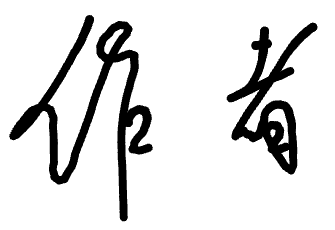
\includegraphics[width=0.5\textwidth]{signatures/author.png}
    \caption{懒得画图了,随便放个签名}
    \label{fig:example}
\end{figure}

\begin{table}[htbp]
    \centering
    \caption{测试表格}
    \begin{tabularx}{0.8\linewidth}{|L|C|R|}
        \hline
        列1  & 列2  & 列3  \\
        \hline
        数据1 & 数据2 & 数据3 \\
        \hline
    \end{tabularx}
    \label{tab:example}
\end{table}

\subsection{测试一下引用}

如图\ref{fig:example}所示,测试一下图片引用。

如表\ref{tab:example}所示,测试一下表格引用。

还有参考文件引用:
引用样式1\cite{example2025}。
引用样式2\parencite{example2025}。

\subsection{测试一下子节}
\subsubsection{测试一下子子节}

\begin{description}
    \item[介绍一个东西] 这里是具体内容描述文本,他需要有一点长。具体需要多长呢,大概需要比一页多一点。这样他就可以换行了。
    \item[介绍另一个] 另一段内容...
\end{description}